\chapter{相关知识}

\section{网络协议}

网络协议是分布式系统与通信网络的基础。为了使网络中不同体系结构的计算机能够准确地交换数据，必须对数据的传输格式、传输速率、步骤等制定统一的规则。这些为进行网络数据交换而建立的规则、标准或约定，统称为网络协议 \cite{tanenbaum2011computer}。

\subsection{协议报文的基本要素}

一个严谨的协议报文定义通常由语法、语义和时序三个基本要素构成。
其中，语法（Syntax）定义了数据与控制信息的结构或格式，包括数据字段的类型、长度、先后顺序以及特定的标识符；语义（Semantics）规定了数据每一部分的具体含义，例如某个字节代表的是“读请求”还是“写请求”，以及如何解释复杂的复合字段；时序（Timing）则指明了实体间通信的顺序，以及由于事件触发而导致的状态演变，即协议状态机。这三个要素共同构成了协议的完整定义，确保了通信双方能够正确理解和处理交换的数据。

\subsection{协议的分类}

根据数据封装与语义解析方式的不同，网络协议主要可分为文本协议（Text-based Protocol）与二进制协议 (Binary Protocol) 两大类。文本协议（如 HTTP、SMTP）使用可读的文本格式进行通信，便于调试和分析；而二进制协议（如 MQTT、DTLS）则使用紧凑的二进制格式，
通常具有更高的效率和更小的消息体积。

\subsection{协议的交互}

网络协议的交互过程主要基于经典的客户端-服务器（Client-Server, C-S）架构。该架构将通信双方划分为两个具有明确职能差异的角色：服务器（Server）与客户端（Client）。服务器作为服务的提供方，通常运行在高性能主机上并处于长期的监听状态，负责管理核心资源并被动等待接入；客户端则作为服务的请求方，根据用户需求主动向服务器发起连接。每一轮交互始于客户端发送的请求报文，服务器在接收并处理该报文后，返回相应的响应报文以完成闭环。在这种架构下，协议的交互具有明显的非对称性：交互的节奏和时机通常由客户端驱动，而服务器则负责处理并发请求并维持服务的稳定性。这种角色分明的设计简化了网络通信的组织形式，使得协议能够高效地实现资源共享与数据交换。

\subsection{协议的特点}

网络协议的核心特性主要体现在结构化的数据表达和严格的行为逻辑两个方面。

首先，在数据表达层面，协议通过定义清晰的报文结构来规定数据的静态布局。各字段具有固定的偏移和边界，从而保证信息交换的确定性。在此基础上，协议进一步通过字段语义约束限定数据项的取值范围，并通过字段之间的依赖关系（如长度字段与校验字段）确保报文整体的一致性与完整性。

其次，在行为逻辑层面，协议具有明显的状态相关性。协议通常通过状态机（State Machine）来描述通信过程中的状态转换，只有在满足特定条件时才会发生状态迁移，从而明确各阶段的转换条件与执行规则，保证通信过程在时序和逻辑上的严谨性。

以图 \ref{fig:proto-stru} 和 图 \ref{fig:proto-state} 所示的 MQTT 协议控制报文为例，其具体的字段布局与状态迁移直观地反映了上述特性。在静态结构上，报文由固定报头中的 \texttt{TYPE} 和 \texttt{FLAG} 起始，紧随其后的是 \texttt{REMAINING LENGTH} 字段、\texttt{VARIABLE HEADER}和 \texttt{PAYLOAD}。每个字段的长度和取值范围都收到了严格的定义和约束。例如，\texttt{CONNECT FLAG} 字段共包含 8 位，每一位都具有特定的语义含义，如第 0 位表示是否使用用户名，第 1 位表示是否使用密码等。此外，这些字段之间还存在相互依赖关系，如 \texttt{REMAINING LENGTH} 字段必须正确反映后续字段的总长度，\texttt{CONNECT FLAG} 字段中的特定位决定了 \texttt{PAYLOAD} 中是否包含用户名和密码等信息。

在动态行为上，MQTT Broker的运行严格受控于状态机的变迁：设备初始处于 \texttt{DISCONNECTED} 状态，必须通过特定的连接序列才能进入 \texttt{CONNECTING} 并最终达到 \texttt{CONNECTED} 状态。如果在任何阶段出现不符合协议规范的报文，设备将立即返回错误响应并断开连接。

\begin{figure}[H]
\centering
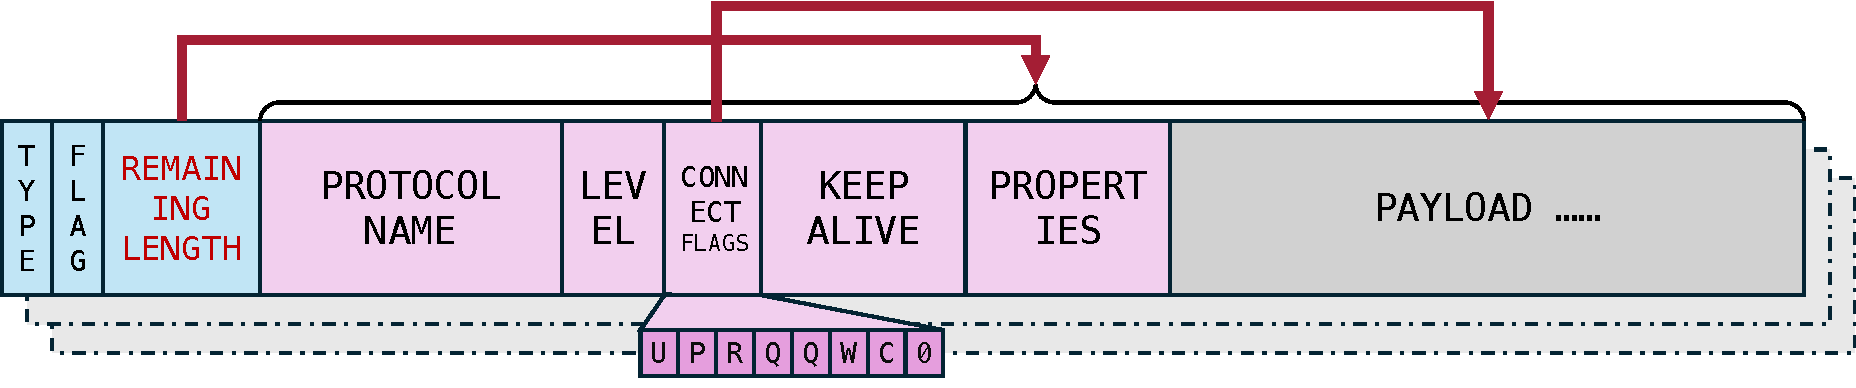
\includegraphics[width=\textwidth]{source/proto-stru.pdf}
\bicaption{MQTT请求消息结构示例}{Example of MQTT Request Message Structure}
\label{fig:proto-stru}
\end{figure}

\begin{figure}[H]
\centering
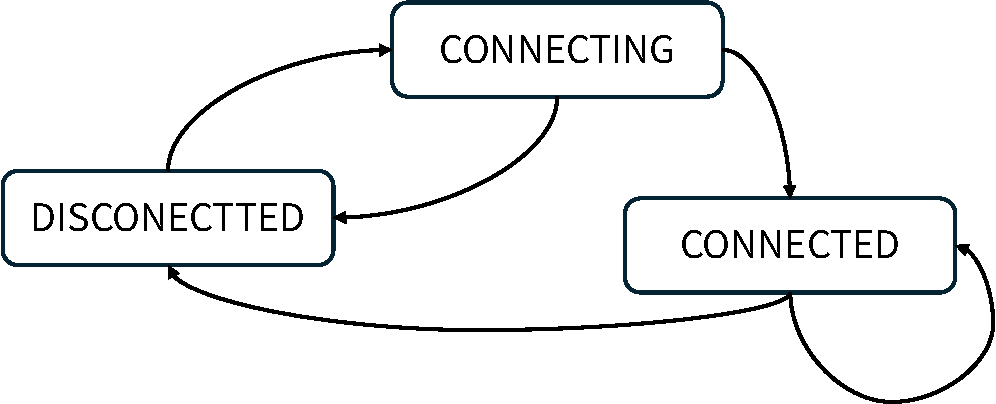
\includegraphics[width=0.5\textwidth]{source/proto-state.pdf}
\bicaption{MQTT协议 Broker 简易状态机示例}{Example of MQTT Broker State Machine}
\label{fig:proto-state}
\end{figure}

\section{模糊测试与协议模糊测试}

模糊测试（Fuzzing）是一种通过向目标程序提供非预期的、随机的或构造的畸形输入，并监测程序是否出现崩溃（Crash）、异常中断、内存泄漏或断言失败等安全漏洞的自动化动态测试技术 \cite{miller1990empirical}。自 20 世纪 80 年代末由 Barton Miller 提出以来，模糊测试凭借其出色的自动化能力和对复杂软件系统的普适性，已成为学术界与工业界挖掘软件漏洞最有效的方法之一 \cite{manes2019art}。

\subsection{模糊测试的基本流程}

一个典型的模糊测试流程通常包含以下五个核心阶段：
\begin{enumerate}[label=\arabic*)]
    \item \textbf{目标分析}：确定被测目标（Target）的输入接口、预期格式、依赖库及执行环境。
    \item \textbf{测试用例生成}：基于特定算法生成初始输入，或从既有的种子语料库（Seed Corpus）中挑选并应用变异算法生成新的测试数据。
    \item \textbf{用例执行}：将生成的测试数据输入目标程序，并触发其运行，通常结合插桩技术以获取运行时信息。
    \item \textbf{状态监控}：实时捕捉程序的运行状态，识别并记录导致程序异常行为的输入样例。
    \item \textbf{结果分析}：对触发异常的测试用例进行去重、精简（Minimizing），并辅助安全研究员溯源漏洞成因。
\end{enumerate}

\subsection{模糊测试的分类}

根据测试过程中对目标程序内部信息的掌握程度，模糊测试主要分为黑盒、白盒与灰盒三类 \cite{liang2018fuzzing}。

\textbf{黑盒模糊测试（Black-box Fuzzing）}。测试者完全不了解程序的内部逻辑或源码，仅通过观测输入与输出的对应关系来发现漏洞。其优点是兼容性强，无需源码，但由于缺乏内部反馈，测试盲目性较高，难以触及深层代码逻辑。

\textbf{白盒模糊测试（White-box Fuzzing）}。通过符号执行（Symbolic Execution）或动态污染分析等技术，系统地探索程序的每一条路径 \cite{godefroid2008automated}。其执行效率虽然较高，但在处理大规模复杂程序时面临严重的“路径爆炸”问题。

\textbf{灰盒模糊测试（Grey-box Fuzzing）}。这是目前学术界与工业界最为主流的范式。它通过轻量级的代码插桩获取程序执行过程中的代码覆盖率（Coverage）反馈，并以此引导变异策略，在测试效率与探索深度之间取得了平衡。代表性工具包括 AFL \cite{zalewski2014american} 及其各类变体。

\subsection{协议模糊测试}

协议模糊测试（Protocol Fuzzing）是将模糊测试技术应用于网络协议实现的一种特定领域的测试方法。与常规的文件模糊测试不同，协议模糊测试的核心在于处理通信过程中的交互性与规范性。有效的模糊测试器必须在生成测试用例时兼顾协议的语法（Syntax）与语义（Semantics），以确保畸形数据能够通过协议解析器的基础校验，从而触达深层的业务处理逻辑。此外，针对具有复杂逻辑的协议，测试工具还需具备状态感知能力，通过模拟合规的状态变迁路径，将测试负载精准投递至特定的协议执行阶段。

根据测试用例产生方式的不同，
现有的协议模糊测试工具主要可归纳为基于变异（Mutation-based）和基于生成（Generation-based）两种范式\cite{manes2019art}。图 \ref{fig:fuzzing-taxonomy} 形象地展示了这两种范式的差异。

\begin{figure}[H]
    \centering
    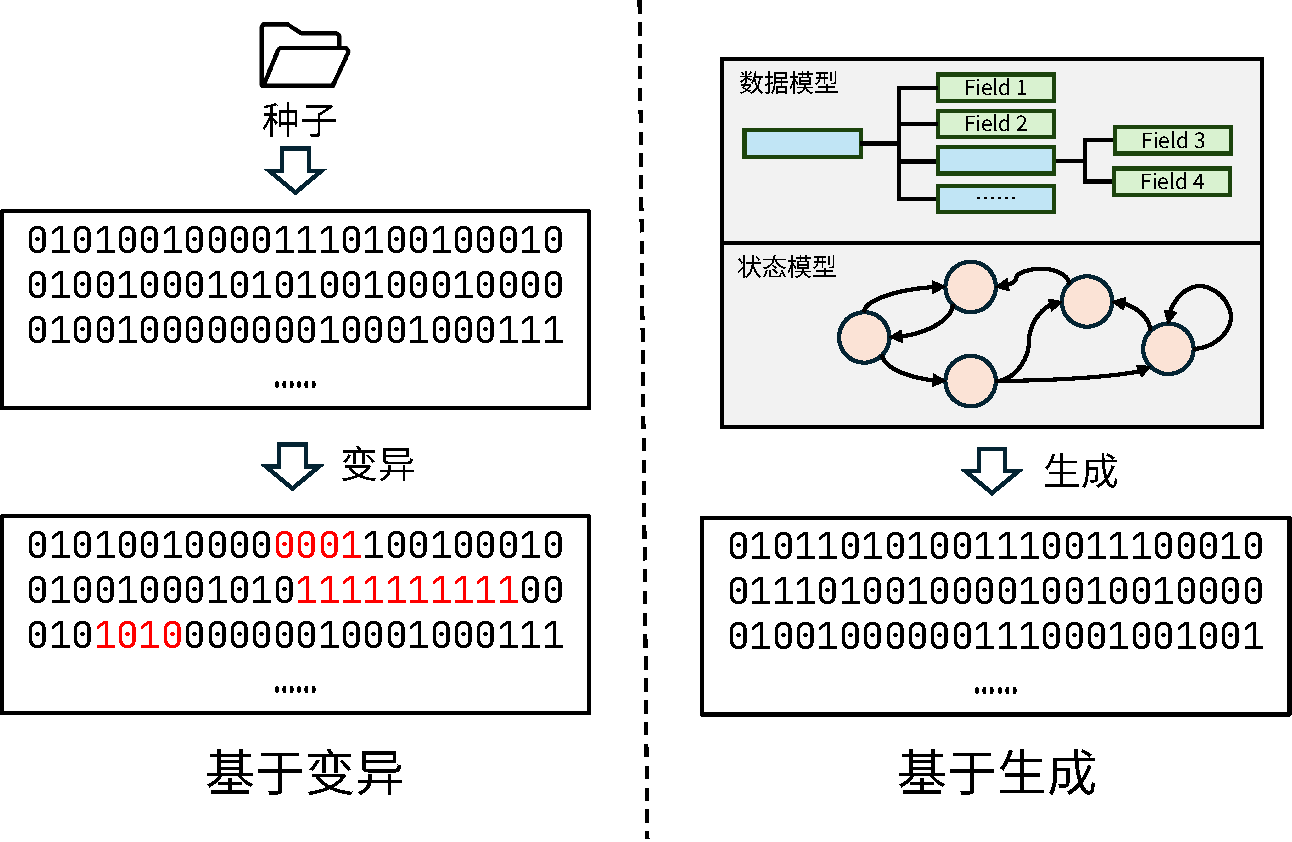
\includegraphics[width=0.7\textwidth]{source/profuzz.pdf}
    \bicaption{协议模糊测试的分类}{Taxonomy of Protocol Fuzzing}
    \label{fig:fuzzing-taxonomy}
\end{figure}

\textbf{基于变异的协议模糊测试}通常不关注协议报文的具体结构，以已知的、合法或半合法的协议通信数据包为起点，通过应用随机或启发式的变异算子（如位翻转、字节替换、数据块插入与删除等）生成大量的测试用例。
这种方法的核心优势在于其较低的部署门槛：测试人员无需深入了解协议的内部细节和规范即可开展测试\cite{zhang2023survey}，尤其适用于缺乏公开文档的私有协议或黑盒测试场景。
然而，网络协议往往具有严格的语法格式和校验机制，简单的盲目变异极易破坏数据包的结构完整性，导致生成的测试用例在协议解析的极早期阶段便被目标程序丢弃，难以触发深层次的代码逻辑和复杂的状态转移。
在基于变异的协议模糊测试工具中，AFLNet\cite{pham2020aflnet}、SGFuzz\cite{ba2022sgfuzz} 和 NSFuzz\cite{qin2023nsfuzz} 是具有代表性的研究工作，它们通过引入状态感知的变异策略和网络环境适应机制，在一定程度上提升了模糊测试的效率和效果。

\textbf{基于生成的协议模糊测试}则要求研究人员对协议的输入格式进行显式的建模，定义协议字段的类型、长度、取值范围以及状态机等信息，以指导测试用例的生成。
模糊测试引擎依据这些预定义的规则和模板，构造出符合协议语法和部分语义规则的数据包。
经典工具如 SPIKE、Sulley 及其衍生的 Boofuzz \cite{boofuzz}，以及基于 XML 建模的 Peach \cite{gitlab_protocol_fuzzer_ce}等，均属于此类。
由于生成的测试数据包在结构上大体符合协议规范，它们能够轻易绕过前期的格式校验逻辑，从而有更高的概率深入探索目标程序的深层逻辑。
尽管有效性较高，但该范式的局限性同样明显：它高度依赖于人工编写协议规范或数据模型，工具的效果也在很大程度上取决于模型的准确性和完整性。
对于庞大复杂的现代网络协议或是未公开的工业控制协议，构建准确且覆盖全面的模型需要耗费巨大的专家人力成本，且工具的通用性和可扩展性较差。

\section{Peach 模糊测试框架}

Peach Fuzzer  \cite{gitlab_protocol_fuzzer_ce} 是一个开源的模糊测试框架，最初在 2004 年前后由 Michael Eddington 开发。它提出了一种基于 XML 建模的通用框架，使得研究人员能够通过编写配置文件（Pit 文件）来描述复杂的协议结构，用于生成和执行模糊测试用例。

目前在安全研究领域广泛使用的 \texttt{gitlab/protocol-fuzzer-ce}，是Peach社区版的一个重要开源维护分支。它保留了 Peach 的核心引擎架构，由于其跨平台性以及对工控协议、网络协议和文件格式的深度支持，至今仍是物联网和工业互联网安全研究中的主力工具之一。

\subsection{核心架构}

Peach 的架构设计遵循高度模块化的原则。如图 \ref{fig:peach_architecture} 所示，整个框架由以下关键组件构成：

\begin{figure}[H]
    \centering
    \includegraphics[width=0.9\textwidth]{source/peach-arch.pdf}
    \bicaption{Peach 模糊测试框架架构图}{Peach Fuzzer Architecture Diagram}
    \label{fig:peach_architecture}
\end{figure}

\begin{enumerate}[label=\arabic*)]
    \item \textbf{Pit 配置文件（Pit File）}：Pit 文件是 Peach 模糊测试框架的核心描述载体，采用 XML 格式对整个测试过程进行声明式建模。它不仅通过 数据模型 精确刻画输入数据的语法结构（包括字段类型、长度约束以及字段间依赖关系），还借助 状态模型 描述协议交互或程序执行的状态迁移逻辑，从而能够表达具有上下文语义的复杂测试流程。此外，Pit 文件还整合了 发布器、监视器 等组件的配置，使测试目标的连接方式与运行时监控机制得以统一描述。这种将测试知识结构化、模块化的设计，使得测试逻辑可以被复用、扩展，并在不同场景下快速迁移。

    \item \textbf{引擎（Engine）}：Peach 引擎是整个模糊测试过程的调度与执行核心，负责解析 Pit 文件并将其转化为可执行的测试流程。在运行过程中，引擎调用变异策略，根据 数据模型 生成符合基本格式约束的测试输入，并结合 状态模型 驱动状态转换，从而实现对目标程序的系统化探索。同时，引擎还负责协调 发布器 进行输入投递，并与 代理/监视器 通信以获取目标程序的运行反馈（如崩溃、异常或挂起）。通过这种集中式控制机制，引擎实现了测试用例生成、执行与结果收集的闭环管理，是连接各功能模块的关键枢纽。

    \item \textbf{代理与监视器（Agent and Monitor）}：代理 与 监视器 共同构成了 Peach 的运行时观测与反馈机制，是实现自动化漏洞检测的重要基础。代理 通常作为独立进程部署在目标环境中，可以是本地或远程系统，其主要职责是加载并管理多个 监视器 组件。不同类型的 监视器 提供了多样化的监控能力，例如调试器型 监视器（如 WindowsDebugger、LinuxDebugger）可以捕获崩溃时的寄存器与调用栈信息，而轻量级 监视器 则可以通过检测进程状态判断程序是否异常终止。一旦检测到错误，监视器 会立即收集相关上下文信息并通过 代理 回传给引擎，从而支持后续的漏洞分析与复现。

    \item \textbf{发布器（Publisher）}：发布器 是 Peach 中用于抽象输入输出操作的关键组件，负责将生成的测试数据传递给目标系统，并在必要时接收响应数据。通过对底层通信机制（如 TCP、UDP、文件系统等）的统一封装，发布器 屏蔽了具体传输细节，使得测试逻辑能够独立于具体执行环境。例如，同一份 数据模型 可以在不做修改的情况下，通过替换 发布器，从网络协议测试切换为文件格式测试。这种解耦设计显著提升了测试模型的通用性与可移植性，同时也便于扩展支持新的通信方式或接口类型。

    \item \textbf{变异器与变异策略（Mutators and Mutation Strategies）}：变异器与变异策略是 Peach 实现输入空间探索的核心机制。变异器定义了具体的修改方式，例如针对数值字段进行边界值替换、对字符串进行插入或截断、或对结构化数据进行重排与嵌套变换等，从而生成具有异常特征但仍满足基本格式约束的测试用例。在此基础上，变异策略则决定了不同变异器的调度方式与应用顺序，例如顺序遍历、随机选择或``确定性随机''。这使得 Peach 能够在保证输入有效性的同时，高效地覆盖更广泛的程序路径，提高发现深层漏洞的概率。
\end{enumerate}

\subsection{数据模型与状态模型}

在 Peach Pit 文件中，数据模型（DataModel）通过层次化的 XML 元素对二进制或文本数据的结构进行精确描述。
其基本构成包括整数（\texttt{Number}）、字符串（\texttt{String}）以及原始数据块（\texttt{Blob}）等基础元素，并支持通过组合这些元素构建复杂的数据结构。
Peach 拥有在一定程度上对字段间语义关系的建模能力，例如通过 \texttt{Relation} 元素自动维护长度字段的一致性，以及借助 \texttt{Fixup} 机制（如 CRC32、MD5）在变异后动态更新校验值。
这种机制保证了生成的测试用例在语法层面依然有效，从而能够穿透目标程序的浅层校验逻辑，触达更深层的执行路径。
此外，Peach 还支持数据解析（Data Cracking），即在接收目标返回数据时，根据既定数据模型将原始字节流反向解析为结构化表示，为后续状态决策与数据依赖提供支持。

图 \ref{fig:dm_example} 展示了一个简单的 UDP 数据包的数据模型示例，其中定义了源端口、目的端口、长度和校验和等字段，并通过 \texttt{Relation} 和 \texttt{Fixup} 元素实现了字段间的约束关系和动态修复机制。

\begin{figure}[H]
\centering
\begin{lstlisting}[numbers=left, frame=single, breaklines=true, basicstyle=\codefont\small, frameround=tttt,rulecolor=\color{black},backgroundcolor=\color{white},belowskip=0pt,numberstyle=\small\color{gray}]
<DataModel name="UdpPacket">
  <Number name="SrcPort" size="16" endian="big" />
  <Number name="DestPort" size="16" endian="big" />
  <Number name="Length" size="16" endian="big">
    <Relation type="size" of="UdpPacket" />
  </Number>
  <Number name="CheckSum" size="16" endian="big" >
    <Fixup class="UDPChecksumFixup">
      <Param name="ref" value="UdpPacket"/>
    </Fixup>
  </Number>
  <Blob name="Data" />
</DataModel>
\end{lstlisting}
\bicaption{数据模型示例}{Example of DataModel}
\label{fig:dm_example}
\end{figure}

状态模型（StateModel）用于描述模糊测试过程中与目标系统的交互流程及其状态演化。
该模型以状态为基本单元，通过一系列动作（Action）定义具体的交互行为，例如 \texttt{output} 用于发送构造的数据，\texttt{input} 用于接收并解析响应，而 \texttt{slurp} 则用于从当前数据流中提取关键字段并存储为内部变量。
在此基础上，状态模型通过显式的状态迁移机制（如 \texttt{changeState}）实现对协议语义的建模，使得后续测试行为能够依据目标反馈动态调整执行路径。
例如，在典型的认证流程中，仅当先前交互满足特定条件时，系统才会进入后续功能状态。
该种状态感知能力有效避免了无效或不符合上下文的测试输入，从而提升了模糊测试的效率与覆盖深度。

图 \ref{fig:sm_example} 展示了一个简单的状态模型示例，其中定义了两个状态：\texttt{InitialState} 和 \texttt{PongPongBack}。在 \texttt{InitialState} 中，系统首先接受输入并解析为数据模型 \texttt{Ping}，然后根据输入内容决定是否切换到 \texttt{PongPongBack} 状态，最后输出相应的数据模型（\texttt{Pong} 或 \texttt{PongPong}）。

\begin{figure}[H]
\centering
\begin{lstlisting}[numbers=left, frame=single, breaklines=true, basicstyle=\codefont\small, frameround=tttt,rulecolor=\color{black},backgroundcolor=\color{white},belowskip=0pt,numberstyle=\small\color{gray}]
<StateModel name="TheStateModel" initialState="InitialState">
  <State name="InitialState">
    <Action type="accept" />
    <Action type="input">
      <DataModel ref="Ping" />
    </Action>
    <!-- Switch states only when input was PINGPING -->
    <Action type="changeState" ref="PongPongBack"
      when="state.actions[1].dataModel.find('PingPingStr') != None" />
    <Action type="output">
      <DataModel ref="Pong" />
    </Action>
  </State>
  <!-- This state is only reached when input was PINGPING -->
  <State name="PongPongBack">
    <Action type="output">
      <DataModel ref="PongPong" />
    </Action>
  </State>
</StateModel>
\end{lstlisting}
\bicaption{状态模型示例}{Example of StateModel}
\label{fig:sm_example}
\end{figure}


\subsection{基本流程}

Peach 框架进行模糊测试时，是以迭代（Iteration）为基本单位的。
图 \ref{fig:peach_workflow} 展示了一个迭代的基本流程。

\begin{figure}[H]
    \centering
    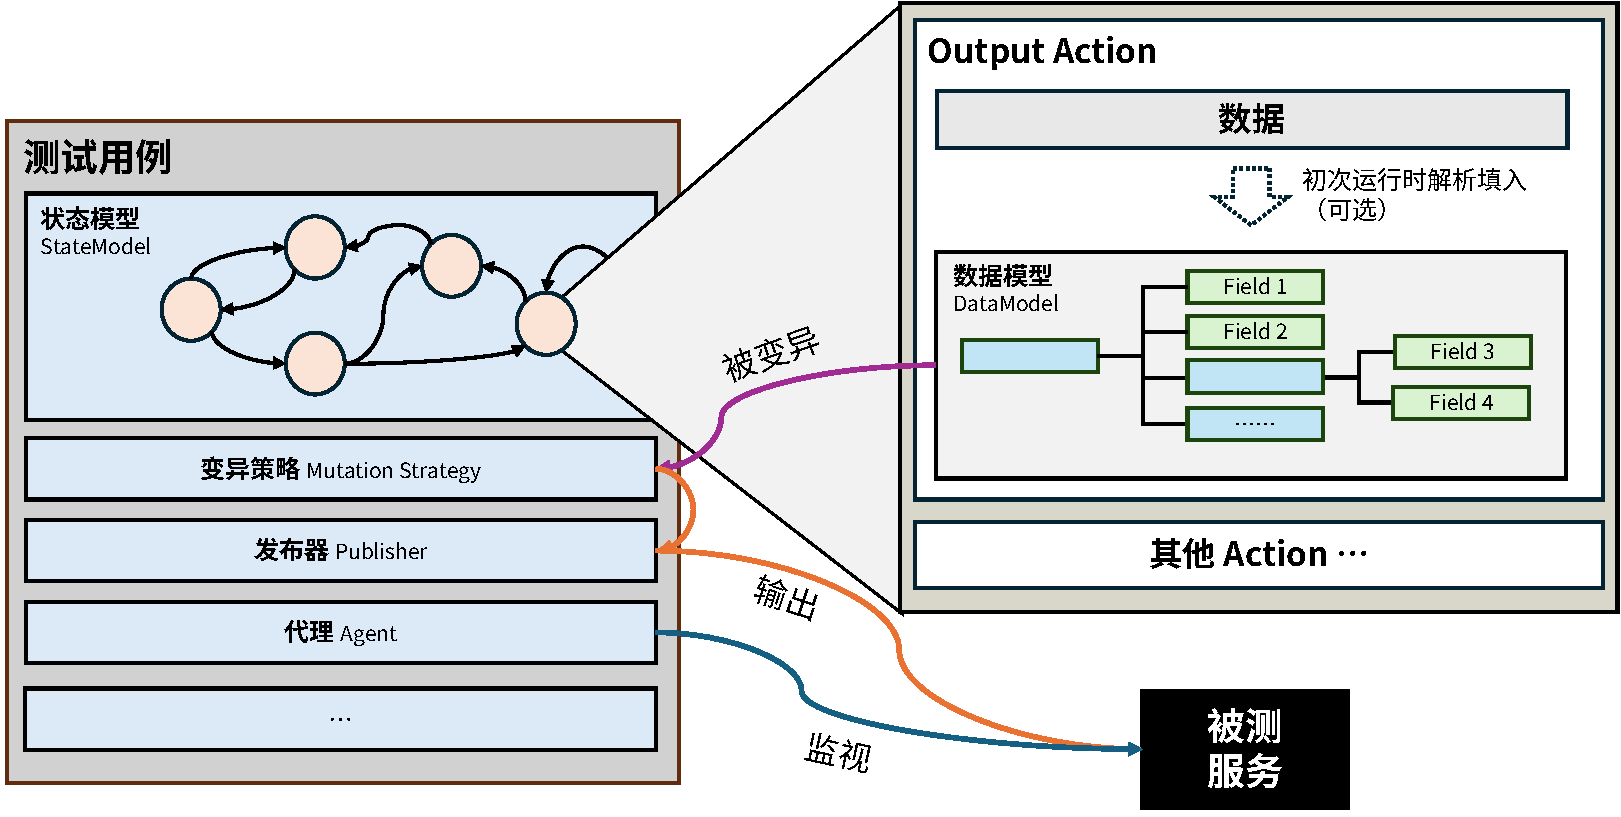
\includegraphics[width=\textwidth]{source/peach.pdf}
    \bicaption{Peach 模糊测试流程示意图}{Peach Fuzzer Workflow Diagram}
    \label{fig:peach_workflow}
\end{figure}

首先，测试用例由 状态模型（StateModel） 与  数据模型（DataModel） 协同定义。
其中，状态模型 描述了测试过程中各个状态之间的转换关系，从而刻画协议交互的时序逻辑；
而 数据模型 则以层次化方式定义了消息的内部结构，包括各字段的类型、长度及约束条件。
此外，如果 测试用例中定义了外部种子数据，则引擎会首先从文件中加载这些数据，并根据数据模型的定义进行解析和结构化处理，填入数据模型中对应的字段位置，作为该字段的默认值。
通过这种结构化建模方式，Peach 能够生成语义上更为合理的初始测试输入，而非简单的字节流拼接。

接着，进行变异生成。变异策略（Mutation Strategy）
组件根据预定义策略，调用相应的变异器，对数据模型中的字段进行扰动。
该过程作用于其数据模型树上的一个或多个字段，生成多样化的测试输入。
变异操作通常不会破坏数据的基本结构（如长度字段与实际数据长度的一致性），使生成的数据在保持结构合法性的同时引入潜在异常。

最后，发布器 （Publisher）
负责将生成的测试用例发送至被测服务，
而 代理（Agent） 则用于监测目标环境中的被测服务。
它持续观察被测服务的运行状态，包括崩溃、异常退出或资源异常等行为。一旦检测到异常，系统将记录对应的测试输入及执行上下文，以便后续分析与漏洞复现。

\subsection{优势与局限性}

Peach 在协议模糊测试领域展现出一些优势。首先，其基于数据模型的语义感知能力使其能够生成符合协议基本结构约束（如长度字段、校验和等）的高质量测试用例，从而显著提高触达目标程序深层逻辑路径的概率。其次，Peach 采用高度模块化的插件式架构，支持用户灵活扩展和定制 变异器、发布器 与 监视器 等核心组件，使其能够适配多样化的测试场景。此外，Peach 提供了完善的状态机建模机制，能够有效支持具有复杂交互流程的有状态协议测试，例如涉及握手、认证及多轮通信的网络协议，这使其在协议层模糊测试中具有较强的表达能力和适用性。

然而，Peach 也存在若干不可忽视的局限性。首先，其对高质量 Pit 文件的依赖导致建模成本较高，用户通常需要深入理解相关协议规范（如 RFC 文档）或借助大量逆向分析工作，这在一定程度上提高了使用门槛。其次，由于 Peach 构建于 .NET/Mono 平台之上，并依赖 XML 进行数据与状态描述，其执行效率相对较低，在每秒执行次数（Exec/s）方面明显逊于 AFL、libFuzzer 等轻量级模糊测试工具。最后，Peach 缺乏基于代码覆盖率的反馈引导机制，本质上属于黑盒模糊测试方法，无法像基于覆盖率反馈的工具那样通过进化策略持续探索新的执行路径，从而在复杂程序中的路径覆盖能力受到一定限制。


\section{大模型智能体}

随着大语言模型（Large Language Models, LLM）的能力不断提升，其应用形态正从单轮文本生成逐步演进为能够执行复杂任务的智能系统。在这一背景下，大模型智能体（LLM Agent）作为一种新兴范式被提出，用以描述以大语言模型为核心，通过与外部环境交互完成多步骤任务的自主系统 \cite{yao2023react,schick2023toolformer}。相比传统仅基于输入输出映射的语言模型，大模型智能体通过引入推理过程建模与工具调用机制，使模型具备一定程度的决策与执行能力，从而能够处理更加复杂和开放的任务场景。

\subsection{基本概念与工作机制}

从系统结构上看，大模型智能体通常运行在一个“感知—推理—行动”的闭环之中。模型首先接收来自外部环境的输入，例如自然语言指令、程序执行结果或结构化数据；随后基于当前上下文进行推理，生成中间思考过程及下一步操作；最后通过调用外部工具或接口执行具体动作，并将执行结果反馈给模型以更新其内部状态。这一过程往往以迭代方式进行，使得模型能够在多轮交互中逐步逼近目标。

这种机制的关键在于将推理过程显式化，使模型不仅输出最终结果，还能够生成中间决策步骤，从而提升复杂任务的可解释性与稳定性。同时，通过引入外部工具（如代码执行器、搜索引擎或数据库接口），大模型智能体能够突破纯文本生成的能力边界，将语言理解与实际操作相结合。


\subsection{挑战与发展趋势}

尽管大模型智能体展现出广泛应用潜力，但其发展仍面临若干挑战。首先，由于大语言模型具有一定的生成不确定性，在多步推理过程中可能出现错误累积，从而影响最终结果的可靠性。其次，工具调用与环境交互通常伴随着额外的计算开销与系统复杂性，这在一定程度上制约了其实际部署效率。此外，大模型智能体的行为在很大程度上依赖于提示设计与控制策略，其泛化能力在不同任务之间仍有待进一步验证。

提升智能体的推理稳定性、降低执行成本，以及构建更加通用且可解释的决策机制，是当前研究的热点方向。
同时，如何将大模型智能体与具体应用领域深度融合，也是推动其落地的重要方向。